%
\documentclass[11pt]{thesis} % draft

\title{Algorithmic Meta-Creativity}
\author{Fania Raczinski}
\date{March 2015}


\begin{document}

\begin{figure}[!htbp] % (here, top, bottom, page)
  \centering
  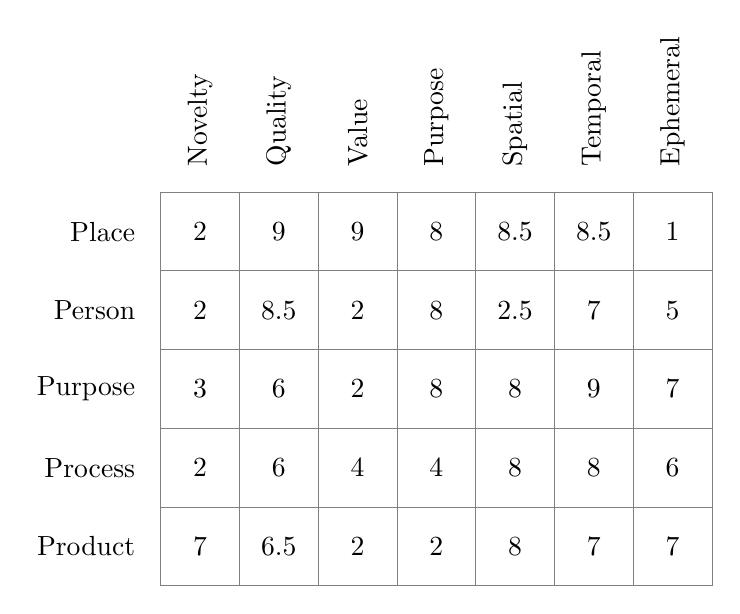
\begin{tikzpicture}
  \draw[help lines] (0,0) grid (7,5);

  \node [anchor=east] at (-0.2,4.5) {Place};
  \node [anchor=east] at (-0.2,3.5) {Person};
  \node [anchor=east] at (-0.2,2.5) {Purpose};
  \node [anchor=east] at (-0.2,1.5) {Process};
  \node [anchor=east] at (-0.2,0.5) {Product};

  \node [rotate=90, anchor=west] at (0.5,5.2) {Novelty};
  \node [rotate=90, anchor=west] at (1.5,5.2) {Quality};
  \node [rotate=90, anchor=west] at (2.5,5.2) {Value};
  \node [rotate=90, anchor=west] at (3.5,5.2) {Purpose};
  \node [rotate=90, anchor=west] at (4.5,5.2) {Spatial};
  \node [rotate=90, anchor=west] at (5.5,5.2) {Temporal};
  \node [rotate=90, anchor=west] at (6.5,5.2) {Ephemeral};

  \node at (0.5,0.5) {7}; % Product Novelty
  \node at (1.5,0.5) {6.5}; % Product Quality
  \node at (2.5,0.5) {2}; % Product Value
  \node at (3.5,0.5) {2}; % Product Purpose
  \node at (4.5,0.5) {8}; % Product Spatial
  \node at (5.5,0.5) {7}; % Product Temporal
  \node at (6.5,0.5) {7}; % Product Ephemeral

  \node at (0.5,1.5) {2}; % Process Novelty
  \node at (1.5,1.5) {6}; % Process Quality
  \node at (2.5,1.5) {4}; % Process Value
  \node at (3.5,1.5) {4}; % Process Purpose
  \node at (4.5,1.5) {8}; % Process Spatial
  \node at (5.5,1.5) {8}; % Process Temporal
  \node at (6.5,1.5) {6}; % Process Ephemeral 

  \node at (0.5,2.5) {3}; % Purpose Novelty
  \node at (1.5,2.5) {6}; % Purpose Quality
  \node at (2.5,2.5) {2}; % Purpose Value
  \node at (3.5,2.5) {8}; % Purpose Purpose
  \node at (4.5,2.5) {8}; % Purpose Spatial
  \node at (5.5,2.5) {9}; % Purpose Temporal
  \node at (6.5,2.5) {7}; % Purpose Ephemeral 

  \node at (0.5,3.5) {2}; % Person Novelty
  \node at (1.5,3.5) {8.5}; % Person Quality
  \node at (2.5,3.5) {2}; % Person Value
  \node at (3.5,3.5) {8}; % Person Purpose
  \node at (4.5,3.5) {2.5}; % Person Spatial
  \node at (5.5,3.5) {7}; % Person Temporal
  \node at (6.5,3.5) {5}; % Person Ephemeral 

  \node at (0.5,4.5) {2}; % Place Novelty
  \node at (1.5,4.5) {9}; % Place Quality
  \node at (2.5,4.5) {9}; % Place Value
  \node at (3.5,4.5) {8}; % Place Purpose
  \node at (4.5,4.5) {8.5}; % Place Spatial
  \node at (5.5,4.5) {8.5}; % Place Temporal
  \node at (6.5,4.5) {1}; % Place Ephemeral 
  \end{tikzpicture}
\caption[Example matrix]{Example matrix}
\label{fig:exmatrix}
\end{figure}



% \newpage

% \chapter{AMC Paradigm}

% A new paradigm for computing sciences that is not AI or robotics or sci-fi but very much to do with true AMC.

% \section{Abstraction}


% To me, the question of whether computers can be intelligent and make ethical decisions includes asking whether a computer can be creative. A lot of the arguments for or against \ac{AI} and computer ethics can be applied to computer creativity.  

% - different levels of abstraction require different levels of study
% - quantum mechanics Heisenberg's uncertainty principle (can't know position and momentum at same time)
% - Schroedinger's cat ``when does a quantum system stop existing as a superposition of states and become one or the other?''



% \section{Creativity, Intelligence and Ethics}

% A more theoretical aspect of this analysis is concerned with what was already discussed to an extent in chapter~\ref{ch:interpretation} (specifically sections~\ref{ss:anthropomorphism}, \ref{s:programmer}, \ref{s:mimicry} and \ref{s:babying}), namely the thread connecting `artificial' creativity, \acl{AI} and `artificial' ethics.

% To me, the question of whether computers can be intelligent and make ethical decisions is the same as asking whether a computer can be creative. A lot of the arguments for or against \ac{AI} and computer ethics can be applied to computer creativity.  

% Answering the question of whether computers can think in my view would also answer the question of whether computers can be creative.


% \subsection{Thinking Computers}
 
% The question of whether computers can think is highly debated and raises many questions. Robert Horn groups the various strands of enquiry related to this question into 8 main arguments \citeyear{Horn2009}. 

% \begin{quotation}
%   \begin{enumerate}
%     \item \textbf{Can computers think?}
%       \begin{itemize}
%         \item Can computers have free will?
%         \item Can computers have emotions?
%         \item Can computers be creative?
%         \item Can computers understand arithmetic?
%         \item Can computers draw analogies?
%         \item Can computers be persons?
%         \item Is the brain a computer?
%         \item Can computers reason scientifically?
%         \item Are computers inherently disabled?
%         \item Should we pretend that computers will never be able to think?
%         \item Does God prohibit computers from thinking?
%       \end{itemize}
%     \item \textbf{Can the Turing test determine whether computers can think?}
%       \begin{itemize}
%         \item Is failing the test decisive?
%         \item Is passing the test decisive?
%         \item If a simulated intelligence passes, is it intelligent?
%         \item Have any machines passed the test?
%         \item Is the test, behaviouraly or operationally construed, a legitimate intelligence test?
%         \item Is the test, as a source of inductive evidence, a legitimate intelligence test?
%         \item Is the neo-Turing test a legitimate intelligence test?
%         \item Does the imitation game determine whether a computer can think?
%         \item Can the Loebner Prize stimulate the study of intelligence?
%         \item Other Turing test arguments
%       \end{itemize}
%     \item \textbf{Can physical symbol systems think?}
%       \begin{itemize}
%         \item Does thinking require a body?
%         \item Is the relation between hardware and software similar to that between human brains and minds?
%         \item Can physical symbol systems learn as humans do?
%         \item Can the elements of thinking be represented in discrete symbolic form?
%         \item Can symbolic representations account for human thinking?
%         \item Does the situated action paradigm show that computers can't think?
%         \item Can physical symbol systems think dialectically?
%         \item Can a symbolic knowledge base represent human understanding?
%         \item Do humans use rules as physical symbol systems do?
%         \item Does mental processing rely on heuristic search?
%         \item Do physical symbol systems play chess as humans do?
%         \item Other physical system arguments
%       \end{itemize}
%     \item \textbf{Can Chinese Rooms think?}
%       \begin{itemize}
%         \item Do humans, unlike computers, have intrinsic intentionality?
%         \item Is biological naturalism valid?
%         \item Can computers cross the syntax-semantics barrier?
%         \item Can learning machines cross the syntax-semantics barrier?
%         \item Can brain simulators think?
%         \item Can robots think?
%         \item Can a combination robot/brain simulator think?
%         \item Can the Chinese Room, considered as a total system, think?
%         \item Do Chinese Rooms instantiate programs?
%         \item Can an internalized Chinese Room think?
%         \item Can translations occur between the internalized Chinese Room and the internalizing English speaker?
%         \item Can computers have the right causal powers?
%         \item Is strong AI a valid category?
%         \item Other Chinese Room arguments
%       \end{itemize}
%     \item \textbf{Can connectionist networks think?}
%       \begin{itemize}
%         \item Are connectionist networks like human neural networks?
%         \item Do connectionist networks follow rules?
%         \item Are connectionist networks vulnerable to the arguments against physical symbol systems?
%         \item Does the subsymbolic paradigm offer a valid account of connectionism?
%         \item Can connectionist networks exhibit systematicity?
%         \item Other connectionist arguments
%       \end{itemize}
%     \item \textbf{Can computers think in images?}
%       \begin{itemize}
%         \item Can images be realistically be represented in computer arrays?
%         \item Can computers represent the analog properties of images?
%         \item Can computers recognize Gestalts?
%         \item Are images less fundamental than propositions?
%         \item Is image psychology a valid approach to mental processing?
%         \item Are images quasi-pictorial representations?
%         \item Other imagery arguments
%       \end{itemize}
%     \item \textbf{Do computers have to be conscious to think?}
%       \begin{itemize}
%         \item Can computers be conscious?
%         \item Is consciousness necessary for thought?
%         \item Is the consciousness requirement solipsistic?
%         \item Can higher-order representations produce consciousness?
%         \item Can functional states generate consciousness?
%         \item Does physicalism show that computers can be conscious?
%         \item Does the connection principle show that consciousness is necessary for thought?
%       \end{itemize}
%     \item \textbf{Are thinking computers mathematically possible?}
%       \begin{itemize}
%         \item Is mechanistic philosophy valid?
%         \item Does G{\"o}del's theorem show that machines can't think?
%         \item Does G{\"o}del's theorem show that machines can't be conscious?
%         \item Do mathematical theorems like G{\"o}del's show that computers are intrinsically limited?
%         \item Does G{\"o}del's theorem show that mathematical insight is non-algorithmic?
%         \item Can automata think?
%         \item Is the Lucas argument dialectical?
%         \item Can improved machines beat the Lucas argument?
%         \item Is the use of consistency in the Lucas argument problematic?
%         \item Other Lucas arguments
%       \end{itemize}
%   \end{enumerate}
%   \sourceatright{\autocite{Horn2009}}
% \end{quotation}

% As early as 1842, Ada Lovelace briefly mentioned the topic in the annotations to her translation of Menabrea's account of Babbage's \textit{Analytical Engine} \autocite{Menabrea1842}. She said the ``Analytical Engine has no pretensions whatever to \textit{originate} anything. It can do \textit{whatever we know how to order it} to perform'', implying that the machine cannot think by itself.

% Alan Turing 


% Alan Turing addressed this question as early as 1951 and .




% \spirals

% \autocite{Turing1951} ``Can digital computers think?''


% ``The more complicated the machine to be imitated the more complicated must the programme be.''\autocite{Turing1951} 




% free-will vs determinism
% ``To behave like a brain seems to involve free will, but the behaviours of a digital computer, when it has been programmed, is completely determined.''\autocite{Turing1951} 

% ``We should be pleased when the machine surprises us, in rather the same way as one is pleased when a pupil does something which he had not been explicitly taught to do.''\autocite{Turing1951} 

% ``If we give the machine a programme which results in its doing something interesting which we had not anticipated I should be inclined to say that the machine \textit{had} originated something, rather than to claim that its behaviour was implicit in the programme, and therefore that the originality lies entirely with us.''\autocite{Turing1951} 





% \paragraph{Free Will}

% In his famous article \textit{Computing Machinery and Intelligence} Turing mentions that a digital computer with a `random element' is ``sometimes described as having free will'' although he adds that he ``would not use this phrase'' himself \autocite{Turing2009}. 




% discrete state machines vs clinamen to create more human system?



% \subsection{Artificial Intelligence}

% Searle against strong ai (watson example...), does that apply to strong artificial creativity? Chinese Room, Turing Test

% Philosopher John Searle and his famous argument against strong \ac{AI} breaks down into the following juxtapositions \autocite{Searle2015, Searle1990}.
 
% \begin{itemize}
%   \item Syntax is not semantics.
%   \item Syntax is observer-relative (subjective).
%   \item Semantics is not intrinsic to syntax.
%   \item Simulation is not duplication.
%   \item Computation is observer-relative (subjective).
%   \item Ontologically subjective topics (such as consciousness or creativity) can be studied in epistemically objective ways.
% \end{itemize}

% % epistemically objectivity (mountain A is higher than mountain B)
% % epistemically subjectvity (mountain A is prettier than mountain B)

% % ontologically objectivity (material world) - observer-independent
% % ontologically subjectivity (money, itch, consciousness) - observer-relative

% % Natural intelligence is observer-independent, intrinsic, conscious!
% % Computer intelligence is observer-relative, not intrinsic




% \begin{quotation}
%   If computation is defined in terms of the assignment of syntax then everything would be a digital computer, because any object whatever could have syntactical ascriptions made to it. You could describe anything in terms of 0's and 1's.

%   The ascription of syntactical properties is always relative to an agent or observer who treats certain physical phenomena as syntactical.\sourceatright{\autocite{Searle1990}}
% \end{quotation}

% \begin{quotation}
%   You can see this if you go back to the Primal Story and remind yourself of the difference between the mechanical computer and Turing's human computer. In Turing's human computer there really is a program level intrinsic to the system and it is functioning causally at that level to convert input to output. This is because the human is consciously following the rules for doing a certain computation, and this causally explains his performance. But when we program the mechanical computer to perform the same computation, the assignment of a computational interpretation is now relative to us, the outside homunculi. And there is no longer a level of intentional causation intrinsic to the system.\sourceatright{\autocite{Searle1990}}
% \end{quotation}

% `Computer' as in its original meaning: a person who computes, ie the programmer rather than the machine

% \begin{quotation}
%   All observer relative phenomena are created by human and animal consciousness but the human or animal consciousness that creates them is not itself observer relative.\sourceatright{\autocite{Searle2015}}
% \end{quotation}

% \begin{quotation}
%   Computation is not a fact of nature. It's a fact of our interpretation.\sourceatright{\autocite{Searle2015}}
% \end{quotation}

% \begin{quotation}
%   And insofar as we can create artificial machines that carry out computations, the computation by itself is never going to be sufficient for thinking or any other cognitive process because the computation is defined purely formally or syntactically. Turing machines are not to be found in nature, they are found in our interpretations of nature.\sourceatright{\autocite{Searle2015}}
% \end{quotation}

% \begin{quotation}
%   Programs are formal or syntactical. Minds have a semantics. The syntax by itself is not sufficient for the semantics.\sourceatright{\autocite{Searle2015}}
% \end{quotation}

% Human are more likely to call something AI than they would call something comp creat.
% people project human values onto machines, and human desires too. so the big bad robot uprising is a fear of what humans would do if they feel superior.

% Gödel's incompleteness theorems said that every non-trivial formal system is either incomplete or inconsistent.

% \begin{quotation}
%   Well, if computation isn’t sufficient for thinking, then what is? What is the relation between the mind and the brain, if it is not the same as the relation of the computer program to the hardware? At least the computational theory of the mind has a solution to the mind-body problem. The mind is to the brain as the computer program is to the computer hardware. If you are rejecting that solution, you owe us an alternative solution.\sourceatright{\autocite{Searle1998}}
% \end{quotation}

% \begin{quotation}
%   All of our mental states, everything from feeling pains to reflecting on philosophical problems, is caused by lower level neuronal firings in the brain. Variable rates of neuron firing at synapses, as far as we know anything about it, provide the causal explanation for all of our mental life. And the mental processes that are caused by neurobiological processes are themselves realized in the structure of the brain. They are higher level features of the brain in the same sense that the solidity of this paper or the liquidity of water is a higher level feature of the system of molecules of which the table or the water is composed.

%   To put this in one sentence, the solution to the traditional mind-body problem is this: Mental states are caused by neurobiological processes and are themselves realized in the system composed of the neurobiological elements.\sourceatright{\autocite{Searle1998}}
% \end{quotation}







% \subsection{Artificial Ethics}

% Bernd Stahl and responsible computing..

% ethics in machines: protocols, networking? is in unethical for a computer to crawl my server without asking? only because it causes traffic which causes delays which impact on me the human.

% ethics in humans because we are social beings and need to coexist


% \subsection{Artificial Creativity}

% Cohen argument against artif. creat? AARON



% \section{Brain vs Machine}

% brain argument against artificial anything?







% \spirals



% \spirals

% \begin{quotation}
%   Cohen is the author of AARON, perhaps the longest-lived and certainly the most creative artificial intelligence program in daily use. Cohen viewed AARON as his collaborator. At times during their decades long relationship AARON was quite autonomous, responsible for the composition, coloring and other aspects of a work; more recently, AARON served Cohen by making drawings that Cohen would develop into paintings. Cohen's death is the end of a lengthy partnership between an artist and an artificial intelligence.\sourceatright{\autocite{Cohen2016}}
% \end{quotation}

% \begin{quotation}
%   Cohen had no patience for the ``is it art?'' question. He showed AARON's work in the world's galleries, museums and science centers -- the Tate, the Stedelijk, the San Francisco Museum of Art, Documenta, the Boston Computer Museum, the Ontario Science Center, and many others. His audiences might have been drawn in by curiosity and the novelty of computer-generated art, but they would soon ask, how can a machine make such marvelous pictures? How does it work? The very questions that Cohen asked himself throughout his career.\sourceatright{\autocite{Cohen2016}}
% \end{quotation}

% \todo{aaron stuff}
% \url{http://collections.vam.ac.uk/name/cohen-harold/6433/}

% \begin{quotation}
%   \ldots we'll be seeing an increasing number of artists turning to robotic art of one sort or another in the next five or ten years. We're already seeing some. It's also a pretty safe bet that for the most part they'll be using off-the-shelf robots; that the ``art'' will be manifested in dreaming up contexts they were never intended for; and the culture's definitions of art will change accordingly.
%   \sourceatright{\autocite{Cohen2007}}
% \end{quotation}

% \begin{quotation}
%   Shouldn't it be possible, I wondered, to write the rules for generating material for a painting and then simply follow the rules?  In this way, it would be almost as if the painting was painting itself; and I would be relieved of the uncertain task of inventing on a day-to-day basis. 

%   That was a little naïve, of course; it simply shifted the burden of invention to another place, another level. I'm still inventing on a day to day basis, but now it's likely to be algorithms for doing particular tasks that I'm inventing.
%   \sourceatright{\autocite{Cohen2007}}
% \end{quotation}

% \begin{quotation}
%   I'd like to end with a couple of observations about AARON's algorithm. Firstly; I think it's fair to say that nothing of what has happened could have happened unless I had drawn upon a lifetime of experience as a colorist.  I've evidently managed to pack all that experience into a few lines of code,  yet nothing in the code looks remotely like what I would have been doing as a painter, and AARON's algorithm isn't something a human artist could apply by hand, so to speak.
%   \sourceatright{\autocite{Cohen2007}}
% \end{quotation}

% \begin{quotation}
%   It's twenty years since I first realized that I could never turn AARON into a colorist by having it emulate my own expertise; in that case simply because it lacked the hardware upon which that expertise depended. Now I have AARON exercising an algorithm that couldn't be emulated by human colorists, presumably because they lack the hardware to do what AARON does. (and by hardware, in this case I mean the intellectual machinery that can build a stable enough representation and juggle enough variables, as AARON does in running the algorithm.) 
%   \sourceatright{\autocite{Cohen2007}}
% \end{quotation}

% \begin{quotation}
%   None of this would be interesting if AARON were an indifferent colorist. But I think I can claim, without undue immodesty, that AARON is a world-class colorist, significantly more inventive and infinitely more productive than I ever was myself. And I conclude that, after decades of expert systems  built to simulate human expertise, AARON has emerged as an expert in its own right. That marks a significant change of state, a change of level, in the never-ending pursuit of autonomy, not merely an incremental change in what the program is able to do. 
%   \sourceatright{\autocite{Cohen2007}}
% \end{quotation}

% \begin{quotation}
%   If I were writing AARON's biography today, I might almost say that AARON was a twinkle in its parent's eye in 1963; it was conceived in 1972 but not born until 2006. It has been a long gestation, and right now the parent is struggling to direct an unruly child, keeping it fed and changing its diapers. He has no idea when the child will be potty-trained, much less how long it will be before it reaches adulthood.
%   \sourceatright{\autocite{Cohen2007}}
% \end{quotation}


% % MOVE TO ANALYSIS
% \begin{quotation}
%   [The use of computers] became an instrument, not of combinatorial accumulation, but of anti-combinatorial reduction. It served not to create combinations but to eliminate them.\sourceatright{\autocite[p.131]{Mathews2005}}
% \end{quotation}


% \spirals


% Where does this project stand in the wider world and the progress of computing, \ac{AI} and creativity? \ac{AI} and robotics is alluring as a research topic because it is so prevelant in Science Fiction. Computer creativity rarely plays a central role though. We can regularly read headlines that tell us that yet another kind of \ac{AI}-bot has won some game against a human player. Or we see videos of some innovative ground-breaking kind of new robot which claims to be near human-like (and yet cannot walk up stairs easily or hold a decent conversation). There are many examples of advances that are hailed as the next big thing which aren't all that great in the grand scheme of things. 

% \subsection{AI}
% % This is also evident in games, for example \ac{VR} and \ac{AR}. The Oculus Rift and similar systems are advertised so much you might believe they are actually about to hit mainstream and every kid will own a \ac{VR} console and headset. Yet they are still way too expensive to be mainstream and motion sickness is also still an issue (and probably always will). These industries are so ``hip'' any publication is seen as the new cool thing without taking into account the history and work that has been done previously in perhaps slightly different disciplines. This is the case for example with a recent article on \ac{VR} sickness and how to compat it. This is a well known problem already---motion sickness already exists in normal games. Similar to epilepsy problems.

% % \todo{find links for motion sickness}
% % \todo{find links for epilepsy}
% % \todo{find links for oculus rift and pokenmon go etc}

% % \ac{AR} has very recently received a massive boom thanks to Pokenmon Go (released in Australia, New Zealand and the USA in July 2016). It has become a phenomenon since then.
% % \todo{find pokemon links}

% What about IBM's Watson\footnote{See \url{http://www.ibm.com/watson/}}, Microsoft's Twitter \ac{AI} chatbot Tay\footnote{See \url{https://web.archive.org/web/20160414074049/https://www.tay.ai/} for an archived version of the original website which is now offline. See also \url{https://twitter.com/tayandyou}, \url{https://www.theguardian.com/technology/2016/mar/24/tay-microsofts-ai-chatbot-gets-a-crash-course-in-racism-from-twitter}, and \url{https://www.theguardian.com/technology/2016/mar/30/microsoft-racist-sexist-chatbot-twitter-drugs}. Wikipedia also has a good article and sources on Tay: \url{https://en.wikipedia.org/wiki/Tay_(bot)}}, Google's AlphaGo\footnote{See \url{https://deepmind.com/alpha-go}} and Hanson Robotics Sophia robot\footnote{See \url{http://www.hansonrobotics.com/}}? How does this relate to my work? Practially of course they are all unrelated. On a deeper level though we can start asking interesting questions. 

% \url{https://www.engadget.com/2016/08/07/ibms-watson-ai-saved-a-woman-from-leukemia/}
% \url{https://xkcd.com/1619/} XKCD WATSON
% \url{http://www.wsj.com/articles/SB10001424052748703407304576154313126987674}

% \begin{description}
%   \item[IBM Watson] Watson is a question answering expert system. It famously won against human Jeopardy! champions in 2011.
%   \item[Microsoft Tay] 
%   \item[Google AlphaGo] AlphaGo is a system for playing the game Go. It won against a top human professional player in 2015.
%   \item[Hansen Sophia]
% \end{description}

% I think these are interesting examples to study since they are supposedly on the forefront of \ac{AI} development. Life-like robots like Sophia still live in the `uncanny valley'. Her voice is creepy and unhuman, her intelligence or her capabilities if understanding conversations are clearly flawed (as shown by her viral remark about supporting genocide).\todo{check} Watson is clever and fast in finding answers for specific questions but he still had problems with humour (e.g. BLAHBLA\todo{find example}) but information lookup is arguably fairly easy and straightforward process within \ac{IR}---sure, it requires processing power and memory storage or access but it is based on simple matching of keywords, not any fancy heuristic algorithms. Microsofts twitter chatbot went viral and users `taught' it nasty swearwords \todo{check} quickly and Microsoft had to take the bot down. It has since apologised although any official documentation on it has disappeared \todo{check}. Google's AlphaGo has been hailed as a breakthrough in \ac{AI} but similar to Watson it is a very targeted and limited program. 

% To me it seems the real breakthrough happens when (and if) the first robots appears which isn't as big as a house, can play Go, Chess and hide-and-seek, geniunely manages to get around he uncanny valley effect, has vast knowledge in his memory for instant information lookup, can hold a normal conversation without causing a war, etc, etc---you get the picture. General \ac{AI} is where it's at. Humans can do all the things we do. Children aren't born with only a single function. Imagine a world where humans only have one specialism and can;t do anything else. Mary is a Chess player but can't move her arms. Bob is a medical diagnosis expert but he can't hold a conversation. Movement, speech, memory---they are all vastly complex systems. And I haven't even touched creativity yet.

% \todo{whats the point im making? how does this relate to my work?}
% Perhpas this `uncanny valley' exists in creativity too. If a robot who looks vaguely human but not quite well enough, or he/she/it sounds almost human but not quite---perhaps if a robot can crack a joke like a human but not quite---perhaps this could be considered uncanny valley too? The philosphical zombies I mentioend in chapter~\ref{ch:interpretation}\marginnote{§~\ref{ch:interpretation}} live in this uncanny valley?

% \todo{p and H creativity for computers?}


% \section{Brains}

% I'm not talking about the beer or the zombie food but rather research into the human brain (or animal brains) and attempts to model it on a computer. 

% The motivation here is that once we understand how the brain works, perhaps we can understand how certain cognitive processes really work and this of course include creativity.

% This is no easy task of course. Chris Chatham talks about ten ``important Differences Between Brains and Computers''\footnote{\url{http://scienceblogs.com/developingintelligence/2007/03/27/why-the-brain-is-not-like-a-co/}} which give a good overview of some of the dificulties of trying to model a brain as is. We can't just do a 1-1 copy.

% \begin{quotation}
%   \begin{enumerate}
%     \item Brains are analogue; computers are digital
%     \item The brain uses content-addressable memory
%     \item The brain is a massively parallel machine computers are modular and serial
%     \item Processing speed is not fixed in the brain; there is no system clock
%     \item Short-term memory is not like RAM
%     \item No hardware/software distinction can be made with respect to the brain or mind
%     \item Synapses are far more complex than electrical logic gates
%     \item Unlike computers, processing and memory are performed by the same components in the brain
%     \item The brain is a self-organising system
%     \item Brains have bodies
%     \item	The brain is much, much bigger than any [current] computer
%   \end{enumerate}
% \sourceatright{Chris Chatham}
% \end{quotation}

% To bring this into perspective Ray Kurzweil claims the brain is capable of $10^{16}$ operations per second \citeyear[p.194]{Kurzweil2013}. Japan's K-computer (the worlds largest super computer as of 2016) currently has that power---10 petaflops. The ``Blue Brain Project'' is aiming to model $10^17$ bytes of memory and $10^{18}$ flops by 2023 \autocite[p.125]{Kurzweil2013}.
% \todo{find k-computer reference}

% There are currently some major research projects going on. One of them is the ``Human Brain Project'' \autocite{Walker2012}.

% \begin{draft}
% quotes:

% Our brain consumes about 30W, the same as an electric light bulb, thousands of times less than a small supercomputer. \autocite[p.17]{Walker2012}

% For environmental and business reasons, vendors have set themselves the goal of containing energy consumption to a maximum of 20 megawatts  \autocite[p.41]{Walker2012}

% the 1 PFlop machine at the Jülich Supercomputing Centre could simulate up to 100 million neurons – roughly the number found in the mouse brain. \autocite[p.41]{Walker2012}

% Cellular-level simulation of the 100 billion neurons of the human brain will require compute power at the exascale (1018 flops). \autocite[p.41-42]{Walker2012}

% 2017 petascale 50petabytes memory + 50 petaflops + <=4MW power

% 2021 exascale 200petabyte memory + 1exaflop

% A second, equally important goal will be to prepare the procurement of the HBP Pre-exascale-supercomputer. By 2017/18, Jülich plans to procure a Big Data-centred system with at least 50 PBytes of hierarchical storage-class memory, a peak capability of at least 50 PFlop/s and a power consumption <= 4 MW. The memory and computational speed of the machine will be sufficient to simulate a realistic mouse brain and to develop first-draft models of the human brain. (The rest of the hardware roadmap targets an exascale machine in 2021/2022 with a capability of 1 EFlop/s and a hierarchical storage-class memory of 200 PB).\footnote{https://www.humanbrainproject.eu/high-performance-computing-platform}

% \end{draft}

% Why Minds Are Not Like Computers \autocite{Schulman2009}
% Software – Hardware == Mind – Brain ??? analogy

% "The power of the computer derives not from its ability to perform complex operations, but from its ability to perform many simple operations very quickly."

% Layers of abstraction in computers:\\
% 1.	user interface\\
% 2.	high level programming language\\
% 3.	machine language\\
% 4.	proessor microarchitecture\\
% 5.	Boolean logic gates\\
% 6.	transistors\\

% layers of abstraction in brain:\\
% 1.	personality?\\
% 2.	Thinking?\\
% 3.	Chemical /electrical signals/activity?\\
% 4.	Divided Brain regions/structure\\
% 5.	Neurons\\
% 6.	Dendrites (input) and axons (output)?\\


% Computers are faster and better than humans in many tasks already.

% \begin{quote}
% "The weaknesses of the computational approach include its assumption that cognition can be reduced to mathematics and the difficulty of including noncognitive factors in creativity." \autocite[p.457]{Mayer1999}
% \end{quote}

% \todo{find references}
% \todo{neural networks and other models based on the brain}

% Perhaps we need to have that complete picture of how the brainw orks in order to understand human creativity. I would argue computer creativity is part of general \ac{AI}, and for general \ac{AI} we need massive amounts of general knoweldge.
% \todo{common sense research}
% \todo{again talk about how this is relevant for my project}


% http://users.ecs.soton.ac.uk/harnad/Papers/Py104/searle.comp.html
% Is the Brain a Digital Computer? John R. Searle
% (1990) Presidential Address to the American Philosophical Association
% \autocite{Searle1990}

% ``Structure of the child machine = Heredetary material\\
% Changes of the child machine = Mutations\\
% Natural selection = Judgement of the experimenter''\autocite{Turing2009} 

% ``Digital computers have often been described as mechanical brains.''\autocite{Turing1951} 


% ``...the wisest ground on which to criticise the description of digital computers as `mechanical brains' or `electronic brains' is that, although they might be programmed to behave like brains, we do not at present know how this should be done.''\autocite{Turing1951} 


% \paragraph{Expert Systems vs General AI}
% Is computer creativity an expert system or does it fall into general \ac{AI}? 

% \paragraph{Machines self-assessing}
% Perhaps there is an argument that if humans are the only entities who can judge whether another human is being creative, then machines should be assessing themselves. This is a paradoxical concepts though. Since machines are products made my humans, they can never be autonomous in that sense. If machines had evolved like other animals besides us this argument might hold but obviously that is not the case.


% \section{Ethical Computers}

% This is currently a big issue for example in self-driving vehicles.
% and has always been a faviroite subject in Science Fiction.


\end{document}
